\documentclass{article}
\usepackage[utf8]{inputenc}
\usepackage{setspace}
\usepackage[margin=1.25in]{geometry}
\usepackage{graphicx}
\graphicspath{{./figures/}}
\usepackage{amsmath,amssymb}
\usepackage{booktabs,longtable,array}
\usepackage{lineno}
\usepackage[hidelinks]{hyperref}
\usepackage{microtype}
\linenumbers
\onehalfspacing
% Generated by manuscript/generate_plant_phenomics_numbers.py; do not edit.
\newcommand{\ManualPoleXMLFiles}{12}
\newcommand{\ManualPoleImages}{61}
\newcommand{\ManualPoleAnnotations}{199}
\newcommand{\ManualPoleUsable}{172}
\newcommand{\ManualPoleUnusable}{27}
\newcommand{\SupportPoleLengthFt}{5}
\newcommand{\SupportPoleLengthCm}{152.4}
\newcommand{\FieldMarkIntervalIn}{35}
\newcommand{\FieldMarkIntervalsPerRow}{4}
\newcommand{\AdjacentRowSpacingIn}{140}
\newcommand{\PoleRepeatabilitySeries}{39}
\newcommand{\PoleRepeatabilityRows}{12}
\newcommand{\PoleRepeatabilityAnnotations}{172}
\newcommand{\PoleRepeatabilityMedianCV}{1.24}
\newcommand{\PoleRepeatabilityMedianCVLo}{0.78}
\newcommand{\PoleRepeatabilityMedianCVHi}{1.99}
\newcommand{\PoleRepeatabilityNinetiethCV}{3.65}
\newcommand{\PoleRepeatabilityBelowFive}{38}
\newcommand{\PoleRepeatabilityMaximumCV}{11.51}
\newcommand{\FieldN}{132}
\newcommand{\FieldPlants}{33}
\newcommand{\FieldRows}{12}
\newcommand{\FieldSingleBias}{2.64}
\newcommand{\FieldSingleMAE}{12.03}
\newcommand{\FieldSingleRMSE}{16.81}
\newcommand{\FieldBayesBias}{2.73}
\newcommand{\FieldBayesMAE}{10.97}
\newcommand{\FieldBayesRMSE}{15.81}
\newcommand{\FieldMAEGain}{1.06}
\newcommand{\FieldMAEGainLo}{-0.16}
\newcommand{\FieldMAEGainHi}{2.39}
\newcommand{\FieldBootstrapReplicates}{20,000}
\newcommand{\FieldEndpointN}{33}
\newcommand{\FieldEndpointSingleBias}{2.78}
\newcommand{\FieldEndpointSingleMAE}{14.45}
\newcommand{\FieldEndpointSingleRMSE}{19.44}
\newcommand{\FieldEndpointBayesBias}{6.17}
\newcommand{\FieldEndpointBayesMAE}{12.38}
\newcommand{\FieldEndpointBayesRMSE}{17.02}
\newcommand{\FieldEndpointGain}{2.08}
\newcommand{\FieldEndpointGainLo}{-1.47}
\newcommand{\FieldEndpointGainHi}{6.82}
\newcommand{\FieldAfterFirstN}{99}
\newcommand{\FieldAfterFirstPlants}{32}
\newcommand{\FieldAfterFirstRows}{12}
\newcommand{\FieldAfterFirstSingleMAE}{12.58}
\newcommand{\FieldAfterFirstBayesMAE}{11.14}
\newcommand{\FieldAfterFirstGain}{1.44}
\newcommand{\FieldAfterFirstGainLo}{-0.21}
\newcommand{\FieldAfterFirstGainHi}{3.26}
\newcommand{\FieldDates}{5}
\newcommand{\FieldCovered}{125}
\newcommand{\FieldCoverage}{94.7}
\newcommand{\FieldIntervalWidth}{75.4}
\newcommand{\FieldIntervalMedianWidth}{67.4}
\newcommand{\FieldCoveredEighty}{115}
\newcommand{\FieldCoverageEighty}{87.1}
\newcommand{\FieldCoverageEightyLo}{79.3}
\newcommand{\FieldCoverageEightyHi}{93.6}
\newcommand{\FieldIntervalWidthEighty}{47.9}
\newcommand{\FieldIntervalWidthEightyLo}{46.9}
\newcommand{\FieldIntervalWidthEightyHi}{49.4}
\newcommand{\FieldCoveredNinetyFive}{125}
\newcommand{\FieldCoverageNinetyFive}{94.7}
\newcommand{\FieldCoverageNinetyFiveLo}{89.4}
\newcommand{\FieldCoverageNinetyFiveHi}{98.6}
\newcommand{\FieldIntervalWidthNinetyFive}{75.4}
\newcommand{\FieldIntervalWidthNinetyFiveLo}{73.5}
\newcommand{\FieldIntervalWidthNinetyFiveHi}{78.3}
\newcommand{\FieldEndpointCovered}{31}
\newcommand{\FieldEndpointCoverage}{93.9}
\newcommand{\FieldEndpointIntervalWidth}{67.0}
\newcommand{\PixelImages}{30}
\newcommand{\PixelInstances}{150}
\newcommand{\PixelMatched}{149}
\newcommand{\PixelDetectionRate}{99.3}
\newcommand{\PixelHeightMAEPx}{29.5}
\newcommand{\PixelHeightBiasPx}{9.4}
\newcommand{\PixelHeightRMSECm}{15.91}
\newcommand{\PixelHeightMAECm}{12.27}
\newcommand{\PixelHeightBiasCm}{3.90}
\newcommand{\PixelHeightCorr}{0.837}
\newcommand{\PixelCmPerPx}{0.415886}
\newcommand{\PixelTopMAEPx}{28.3}
\newcommand{\PixelRootMAEPx}{18.2}
\newcommand{\PoleDevCameras}{6}
\newcommand{\PoleDevN}{1083}
\newcommand{\PoleDevMAEIn}{0.186}
\newcommand{\PoleDevMAELoIn}{0.156}
\newcommand{\PoleDevMAEHiIn}{0.218}
\newcommand{\PoleTestCameras}{3}
\newcommand{\PoleTestN}{427}
\newcommand{\PoleTestMAEIn}{0.208}
\newcommand{\PoleTestMAELoIn}{0.158}
\newcommand{\PoleTestMAEHiIn}{0.262}
\newcommand{\DownAllN}{2162}
\newcommand{\DownAllImages}{394}
\newcommand{\DownAllCameras}{10}
\newcommand{\DownAllBiasCm}{0.04}
\newcommand{\DownAllMAECm}{2.20}
\newcommand{\DownAllRMSECm}{5.37}
\newcommand{\DownAllCameraBiasCm}{0.58}
\newcommand{\DownAllCameraMAECm}{2.93}
\newcommand{\DownAllCameraRMSECm}{6.78}
\newcommand{\DownAllCameraMAELoCm}{1.86}
\newcommand{\DownAllCameraMAEHiCm}{4.64}
\newcommand{\DownOneBandN}{1110}
\newcommand{\DownOneBandImages}{394}
\newcommand{\DownOneBandCameras}{10}
\newcommand{\DownOneBandBiasCm}{0.07}
\newcommand{\DownOneBandMAECm}{1.46}
\newcommand{\DownOneBandRMSECm}{3.15}
\newcommand{\DownOneBandCameraBiasCm}{0.40}
\newcommand{\DownOneBandCameraMAECm}{1.91}
\newcommand{\DownOneBandCameraRMSECm}{3.95}
\newcommand{\DownOneBandCameraMAELoCm}{1.24}
\newcommand{\DownOneBandCameraMAEHiCm}{2.98}
\newcommand{\PoleDailyImages}{438}
\newcommand{\PoleDailyPassing}{376}
\newcommand{\AssembledImages}{391}
\newcommand{\AssembledRows}{2283}
\newcommand{\AssembledCameras}{9}
\newcommand{\AssembledPlants}{54}
\newcommand{\PoleStreamRows}{1686}
\newcommand{\PoleStreamForecasts}{1638}
\newcommand{\PoleStreamPlants}{48}
\newcommand{\PoleStreamCameras}{8}
\newcommand{\PoleStreamImages}{330}
\newcommand{\GuessedCoverage}{88.6}
\newcommand{\CalibratedCoverage}{96.4}
\newcommand{\GuessedWidth}{66.6}
\newcommand{\GuessedMedianWidth}{64.6}
\newcommand{\CalibratedWidth}{98.1}
\newcommand{\CalibratedMedianWidth}{93.8}
\newcommand{\ProcessHeightSD}{16.866}
\newcommand{\OutlierProbability}{0.0512}
\newcommand{\OutlierSD}{70.62}
\newcommand{\CalibrationIntervals}{1172}
\newcommand{\CalibratedWIS}{8.08}
\newcommand{\CalibratedLogScore}{-4.440}
\newcommand{\UncertaintyDevN}{1266}
\newcommand{\UncertaintyDevCameras}{6}
\newcommand{\UncertaintyDevPlants}{36}
\newcommand{\UncertaintyDevWIS}{7.93}
\newcommand{\UncertaintyTestN}{372}
\newcommand{\UncertaintyTestCameras}{2}
\newcommand{\UncertaintyTestPlants}{11}
\newcommand{\UncertaintyTestBias}{0.73}
\newcommand{\UncertaintyTestMAE}{15.58}
\newcommand{\UncertaintyTestRMSE}{22.89}
\newcommand{\UncertaintyTestWIS}{8.60}
\newcommand{\UncertaintyTestLogScore}{-4.486}
\newcommand{\UncertaintyDevCoverageFifty}{63.7}
\newcommand{\UncertaintyDevWidthFifty}{30.7}
\newcommand{\UncertaintyTestCoverageFifty}{65.1}
\newcommand{\UncertaintyTestWidthFifty}{30.6}
\newcommand{\UncertaintyDevCoverageEighty}{87.8}
\newcommand{\UncertaintyDevWidthEighty}{59.4}
\newcommand{\UncertaintyTestCoverageEighty}{86.3}
\newcommand{\UncertaintyTestWidthEighty}{59.3}
\newcommand{\UncertaintyDevCoverageNinety}{94.1}
\newcommand{\UncertaintyDevWidthNinety}{78.4}
\newcommand{\UncertaintyTestCoverageNinety}{92.7}
\newcommand{\UncertaintyTestWidthNinety}{78.2}
\newcommand{\UncertaintyDevCoverageNinetyFive}{96.8}
\newcommand{\UncertaintyDevWidthNinetyFive}{98.2}
\newcommand{\UncertaintyTestCoverageNinetyFive}{94.9}
\newcommand{\UncertaintyTestWidthNinetyFive}{97.8}
\newcommand{\UncertaintyTestMedianWidthNinetyFive}{94.2}
\newcommand{\ForecastBayesMAE}{15.13}
\newcommand{\ForecastBayesRMSE}{21.34}
\newcommand{\ForecastLastMAE}{16.64}
\newcommand{\ForecastLastRMSE}{23.63}
\newcommand{\ForecastLinearMAE}{19.95}
\newcommand{\ForecastLinearRMSE}{27.52}
\newcommand{\CausalPrefixes}{391}
\newcommand{\CausalRows}{51,035}
\newcommand{\CausalMismatches}{0}
\newcommand{\PriorNoneRMSE}{10.48}
\newcommand{\PriorPostRMSE}{8.61}
\newcommand{\PriorInsideRMSE}{6.01}
\newcommand{\PriorInsideReduction}{42.7}
\newcommand{\PriorSimulationPlants}{480}
\newcommand{\PriorSimulationScenarios}{8}
\newcommand{\PriorSpuriousProbability}{0.30}
\newcommand{\PriorTruthSelectionRate}{97.0}
\newcommand{\PriorNoneRMSELo}{9.84}
\newcommand{\PriorNoneRMSEHi}{11.13}
\newcommand{\PriorPostRMSELo}{8.07}
\newcommand{\PriorPostRMSEHi}{9.16}
\newcommand{\PriorInsideRMSELo}{5.47}
\newcommand{\PriorInsideRMSEHi}{6.57}
\newcommand{\PriorVsPostGain}{2.60}
\newcommand{\PriorVsPostGainLo}{2.00}
\newcommand{\PriorVsPostGainHi}{3.20}
\newcommand{\RealAuditN}{63}
\newcommand{\RealAuditCameras}{6}
\newcommand{\RealAuditTracks}{17}
\newcommand{\RealAuditAgreement}{100.0}
\newcommand{\RealAuditSingleMAE}{13.38}
\newcommand{\RealAuditPostMAE}{13.07}
\newcommand{\RealAuditPriorMAE}{13.07}
\newcommand{\RealAuditSingleRMSE}{18.01}
\newcommand{\RealAuditPostRMSE}{17.72}
\newcommand{\RealAuditPriorRMSE}{17.72}
\newcommand{\FieldEWMABias}{-9.78}
\newcommand{\FieldEWMAMAE}{14.98}
\newcommand{\FieldEWMARMSE}{20.16}
\newcommand{\FieldEWMAGain}{4.01}
\newcommand{\FieldEWMAGainLo}{1.48}
\newcommand{\FieldEWMAGainHi}{6.73}
\newcommand{\FieldMedianBias}{-12.15}
\newcommand{\FieldMedianMAE}{18.77}
\newcommand{\FieldMedianRMSE}{27.14}
\newcommand{\FieldMedianGain}{7.80}
\newcommand{\FieldMedianGainLo}{3.83}
\newcommand{\FieldMedianGainHi}{12.68}
\newcommand{\FieldHoltBias}{-8.09}
\newcommand{\FieldHoltMAE}{14.04}
\newcommand{\FieldHoltRMSE}{19.25}
\newcommand{\FieldHoltGain}{3.08}
\newcommand{\FieldHoltGainLo}{0.77}
\newcommand{\FieldHoltGainHi}{5.48}
\newcommand{\FieldGaussianBias}{2.74}
\newcommand{\FieldGaussianMAE}{11.62}
\newcommand{\FieldGaussianRMSE}{16.52}
\newcommand{\FieldGaussianGain}{0.66}
\newcommand{\FieldGaussianGainLo}{-0.43}
\newcommand{\FieldGaussianGainHi}{1.79}
\newcommand{\FrozenMatches}{1970}
\newcommand{\SequentialMatches}{2018}
\newcommand{\SequentialExtraMatches}{48}
\newcommand{\FrozenTrackDistance}{0.0396}
\newcommand{\SequentialTrackDistance}{0.0283}
\newcommand{\PosteriorRootChanged}{1963}
\newcommand{\SimulationScenarios}{9}
\newcommand{\SimulationPlantsPerScenario}{60}
\newcommand{\SimulationRMSEMin}{9.07}
\newcommand{\SimulationRMSEMax}{18.07}
\newcommand{\SimulationCoverageMin}{80.0}
\newcommand{\SimulationCoverageMax}{98.5}


\newcolumntype{L}[1]{>{\raggedright\arraybackslash}p{#1}}
\renewcommand{\thesection}{S\arabic{section}}
\renewcommand{\thesubsection}{\thesection.\arabic{subsection}}
\renewcommand{\thefigure}{S\arabic{figure}}
\renewcommand{\thetable}{S\arabic{table}}
\renewcommand{\theequation}{S\arabic{equation}}

\title{Supplementary Materials for\\
Bayesian Longitudinal Maize Height Estimation with Prior-Guided Image Analysis}

\author{Haoming Wang, Chong Wang, Yawei Li, Cheng-Ting Yeh,\\
Patrick S. Schnable, and Peng Liu\\[0.6em]
\small Iowa State University, Ames, Iowa, USA\\
\small Address correspondence to: pliu@iastate.edu}
\date{}

\begin{document}
\maketitle

\noindent This document provides the detailed implementation specification, causal information-set definition, calibration derivation, uncertainty calibration, candidate-selection audit, annotation provenance, and plant-level endpoint results supporting the longitudinal analysis in the main article. It contains no separate reference list; citations and bibliographic details are given in the main article.

\section{Detailed implementation specification}
\label{sec:s-specification}

\subsection{What is and is not Bayesian in the field implementation}

Two sequential operations must be distinguished. The field association code maintains a running horizontal position and base row for each plant. It uses a fixed update gain of 0.5 and does not propagate a position covariance, calculate a data-dependent Kalman gain, or retain position particles. This is a fixed-gain state update, algebraically equivalent to a steady-state Kalman-mean recursion after the gain has been specified. It is not a full Bayesian posterior over position.

The height and growth component is Bayesian. A weighted particle approximation represents the joint distribution of latent height and growth rate. Particles are propagated through the transition model, weighted with the inlier/outlier measurement likelihood, normalized, and resampled when the effective sample size crosses its prespecified threshold. Posterior summaries and one-step predictive distributions are calculated from those weighted particles.

The term \emph{prior-guided image analysis} refers to feedback across the image/model boundary, not simply to the presence of priors in a Bayesian model. The stronger mechanism in which the predicted height distribution re-ranks competing top-keypoint candidates is evaluated in the controlled candidate-ambiguity simulation and in a matched real-image audit. It was not the top-keypoint rule used to produce the primary field-height results. Thus the field implementation supports claims about prior-guided plant association and base-keypoint updating, while the simulation establishes that a height prior can improve top-candidate choice under known ambiguity. The real-image audit tests whether the available natural candidate sets actually contain that ambiguity.

\begin{longtable}{L{2.45cm}L{4.05cm}L{3.25cm}L{3.25cm}}
\caption{Full parameter and implementation specification for the two empirical analysis streams. A dash indicates that the operation was not applied in that stream.}\label{tab:s-parameters}\\
\toprule
Component & Quantity or operation & 2024--2025 daily pole stream & 2021 primary manual-reference validation \\
\midrule
\endfirsthead
\multicolumn{4}{l}{\textit{Table \thetable{} continued}}\\
\toprule
Component & Quantity or operation & 2024--2025 daily pole stream & 2021 primary manual-reference validation \\
\midrule
\endhead
\midrule
\multicolumn{4}{r}{\textit{Continued on next page}}\\
\endfoot
\bottomrule
\endlastfoot

Observation unit & Plant identity and chronological key & \texttt{camera\_genotype}, left-to-right plant track, capture time & \texttt{rowid} plus \texttt{plantid}, field date \\
Observation unit & Measurement entering height filter & Depth-corrected red-band pole calibration, cm & Archived single-image mask extent \texttt{height\_sam}, multiplied by the recorded geometric scale \\
Reference & In-scene physical definition & Red-band pole; adjacent band edges 1 ft (30.48 cm) apart & Camera-support pole annotation is an installation asset, not the source of \texttt{height\_sam} \\
Reference & Depth factor & $D_{\mathrm{tgt}}/D_{\mathrm{ref}}=8.5/10.0=0.85$ & Separate 2021 scale, \PixelCmPerPx{} cm/pixel, zero intercept \\
Calibration history & Reference selection & Best passing calibration with timestamp no later than the current image; fit RMSE capped at 0.5 in & Not applicable to archived \texttt{height\_sam} \\

Field association & Expected plants & 6 per initialized camera view & Archived identities supplied \\
Field association & Initialization & First complete six-detection frame, sorted left to right & -- \\
Field association & Assignment & Minimum total absolute horizontal distance; maximum normalized distance 0.16 & -- \\
Field association & Position/base update & $m_t=(1-K)m_{t-1}+Kx_t$, fixed $K=0.5$; no covariance state & -- \\
Field association & Empirical diagnostic & \SequentialMatches{} matches, \SequentialExtraMatches{} more than frozen first-frame anchors & -- \\

Particle filter & Latent state & Height $h_t$ and growth rate $r_t$ & Same \\
Particle filter & Transition order & Propagate $h_t$ using $r_{t-1}$, then update $r_t$ & Same \\
Particle filter & Number of particles & 5000 & 5000 \\
Particle filter & Base random seed & 20260723; deterministic plant-specific seed from SHA-256 of plant label and base seed & 20260724; same deterministic derivation \\
Particle filter & Initial height & $N(Y_1,\sigma_1^2)$, clipped to $[0,450]$ cm & Same \\
Particle filter & Initial growth & $N(3,2^2)$ cm/day, clipped & $N(0,8^2)$ cm/day, clipped \\
Particle filter & Height limits & 0--450 cm & 0--450 cm \\
Particle filter & Growth limits & -4--15 cm/day & -4--15 cm/day \\
Particle filter & Height-process SD & \ProcessHeightSD{} cm/$\sqrt{\mathrm{day}}$, estimated from depth-corrected 2024 daily increments & 8.78 cm/$\sqrt{\mathrm{day}}$, robust scale of 2021 image increments \\
Particle filter & Growth-process SD & 0.35 cm/day/$\sqrt{\mathrm{day}}$ & 0.35 cm/day/$\sqrt{\mathrm{day}}$ \\
Particle filter & Growth-rate evolution & Random walk ($\rho=1$) & Nonparametric rate-versus-height field from 2024--2025 pole-stream increments; field adopted before growth noise is added \\
Particle filter & Outlier probability $\pi$ & \OutlierProbability{} & 0.065 \\
Particle filter & Outlier SD & \OutlierSD{} cm & 59.04 cm \\
Particle filter & Resampling rule & Systematic resampling when ESS $<0.5M$ & Same \\
Particle filter & Posterior interval & Weighted 0.025 and 0.975 height-particle quantiles after the current image & Same \\
Particle filter & Predictive interval & Numerical 0.025 and 0.975 quantiles of the complete particlewise Gaussian mixture & Same algorithm; field-height comparison emphasizes the posterior interval \\

Measurement SD & Inlier scale & Prespecified root-sum-of-squares budget: 8-cm pose term, pole-fit term, 1.5 cm per band outside fitted range, and band-regularity term; the total is multiplied by 0.85 after depth correction & $12[1+1.5g_t]$ cm, where $g_t$ is the observed gust normalized over the five evaluated dates; range 12--30 cm, fallback 15 cm \\
Measurement SD & Interpretation & Pilot uncertainty model; process and measurement variation are not separately identified & Retrospective full-window weather normalization; prospective use requires externally frozen normalization limits \\

Primary comparison & Empirical sample & Next image-derived measurements after each first observation & All \FieldN{} records, \FieldPlants{} plants, \FieldRows{} rows, and \FieldDates{} dates \\
Primary comparison & Cluster uncertainty & Cameras for calibration summaries & 20,000 row-bootstrap replicates; seed 20260908 (endpoint seed 20260909) \\
\end{longtable}

\section{Causal online definition}
\label{sec:s-causal}

Let $I_t$ be the image acquired at time $t$, and let $\mathcal I_{\leq t}=\{I_1,\ldots,I_t\}$ denote the accumulated image pool. With detector weights, thresholds, reference definitions, geometry, and filter settings fixed, the operational update is
\begin{equation}
\mathcal O_t=A\!\left(I_t,\mathcal O_{t-1};\theta_{\mathrm{fixed}}\right),
\qquad
\mathcal O_t\ \text{is measurable with respect to}\ \mathcal I_{\leq t}.
\label{eq:s-causal-map}
\end{equation}
Here $\mathcal O_t$ contains the association state, physical image measurement, and height-growth particle distribution returned immediately after $I_t$ is added. An image $I_{t+k}$, $k>0$, is absent from Equation~\ref{eq:s-causal-map}. When it arrives, it initiates a new update; it does not revise $\mathcal O_t$.

The field association step predicts each track by carrying forward its running horizontal position $m^x_{t-1}$ and base row $m^b_{t-1}$. Current detections are assigned to these carried states by minimum-cost matching. For an accepted observation $(x_t,b_t)$,
\begin{align}
m^x_t &= (1-K)m^x_{t-1}+Kx_t,\\
m^b_t &= (1-K)m^b_{t-1}+Kb_t, \qquad K=0.5.
\label{eq:s-fixed-gain}
\end{align}
Equation~\ref{eq:s-fixed-gain} stores means only. The code does not store a position covariance, so $m^x_t$ and $m^b_t$ are called running position states rather than position posteriors in this supplement.

The physical reference attached to a plant image is also selected as of $t$: only accepted reference fits whose calibration time is no later than the plant-image capture time are eligible. The selected top and base pixels are converted to centimeters, the depth factor is applied, and the resulting measurement updates the height-growth particle distribution. The cached detection-to-measurement audit recomputed \CausalPrefixes{} camera-time prefixes and compared \CausalRows{} previously emitted rows, with \CausalMismatches{} mismatches.

This prefix audit does not imply that every model-development action occurred prospectively. The primary manual-reference validation uses 2021 plants from 12 stationary-camera rows, with manual height excluded from the image measurement, growth field, filter, noise parameters, and comparator settings. The growth field is transferred from 2024--2025, so this label-held-out, subject-disjoint physical-height validation is retrospective in calendar direction. The separate 2024 development to subject-disjoint 2025 test supplies the secondary early-to-late uncertainty check. A prospective deployment must freeze the wind-normalization range, growth field, detector, gates, and all hyperparameters before the first test image.

In the simulation-only candidate extension, candidate $j$ with detector evidence $c_{tj}$ and implied height $y_{tj}$ is scored before the measurement update as
\begin{equation}
j_t^*=\arg\max_j\left\{c_{tj}\,p(y_{tj}\mid\mathcal I_{\leq t-1})\right\}.
\label{eq:s-candidate-score}
\end{equation}
This operation lets the height prior affect which top candidate becomes the measurement. It is distinct from applying the particle filter after an independently chosen detection, and it was not used to generate the empirical field-height table.

\section{Manual 2021 support-pole annotations}
\label{sec:s-support-poles}

Haoming Wang manually created the physical-reference annotations. The source annotation directory contains one CVAT XML file for each of 12 camera rows, named \texttt{C-XXX.xml}. An XML can contain multiple dated images, and each image can contain several polylines labeled \texttt{pole1} through \texttt{pole4}. These labels distinguish visible camera-support poles within an image. The numeric suffix does not specify pole depth or physical length.

For each polyline, the importer reads all vertices, takes the smallest image row as the nominal camera-mount endpoint and the largest image row as ground contact, and records the sum of segment lengths in pixels. The physical definition is the nominal vertical distance from ground contact to the camera mounting or optical-center height: \SupportPoleLengthFt{} ft (\SupportPoleLengthCm{} cm). Annotation status is read from the CVAT attribute named \texttt{status}. The imported data contain \ManualPoleAnnotations{} traces: \ManualPoleUsable{} marked usable and \ManualPoleUnusable{} marked unusable.

An earlier export contained two filenames for the same C-039 scene. Following the project decision, \texttt{C-039\_2021-07-30.JPG} was retained and \texttt{C-039\_2021-07-30JPG.JPG} was removed. The updated \texttt{C-039.xml} also includes \texttt{LH54.21-C-039\_2021-07-12-10-57\_CAM827.JPG}. The curated source therefore contains \ManualPoleImages{} unique XML-referenced images, and every referenced image was found in the source image directory.

The installation records separately specify four horizontal field-layout intervals of \FieldMarkIntervalIn{} in, totaling \AdjacentRowSpacingIn{} in between adjacent rows. These are not graduations on the vertical support poles. They also differ from the 1-ft red-band spacing on the 2024--2025 calibration poles. The 2021 import is consequently an installation and annotation resource; it is not pooled with red-band calibration observations.

The importer writes three canonical products:
\begin{itemize}
\item \path{data/processed/manual_poles_2021/manual_pole_annotations_2021.csv}, one row per retained trace;
\item \path{data/processed/manual_poles_2021/pole_definitions_2021.csv}, the physical definitions and source records; and
\item \path{data/processed/manual_poles_2021/summary.json}, counts, duplicate decision, and image-presence audit.
\end{itemize}

\section{Physical calibration and depth correction}
\label{sec:s-calibration}

The 2024--2025 red-band pole supplies positions with known 30.48-cm spacing. Within one reference image, band image rows $y_j$ are centered and scaled as $u_j=(y_j-\bar y)/s_y$, and the calibration curve is
\begin{equation}
z(y)=\frac{au+b}{cu+1}.
\label{eq:s-projective}
\end{equation}
Only height differences are used. Consequently, an arbitrary additive physical datum along the pole does not affect a top-minus-base extent. Held-out bands evaluate interpolation, while the root-direction diagnostic removes lower bands, fits retained upper bands, and predicts downward. The reverse lower-to-upper calculation is not evidence about root extrapolation.

For the depth correction, place a camera at physical height $H$. Under the ideal pinhole model with negligible roll and a level shared ground plane, the image row of a point at height $z$ and horizontal distance $D$ can be written, up to the image-row sign convention, as
\begin{equation}
y(z,D)-y_{\mathrm{hor}}=f_{\mathrm{px}}\frac{H-z}{D}.
\label{eq:s-pinhole}
\end{equation}
For two points separated by a vertical extent $h=z_{\mathrm{top}}-z_{\mathrm{base}}$, subtraction removes $H$ and the horizon row:
\begin{equation}
\left|\Delta y(D)\right|=\frac{f_{\mathrm{px}}}{D}h.
\label{eq:s-extent}
\end{equation}
A scale learned at reference depth $D_{\mathrm{ref}}$ would assign a target pixel extent the value
\begin{equation}
h_{\mathrm{pole\ scale}}
=\frac{D_{\mathrm{ref}}}{f_{\mathrm{px}}}\left|\Delta y(D_{\mathrm{tgt}})\right|
=\frac{D_{\mathrm{ref}}}{D_{\mathrm{tgt}}}h_{\mathrm{target}}.
\label{eq:s-depth-bias}
\end{equation}
Therefore,
\begin{equation}
h_{\mathrm{target}}
=\kappa h_{\mathrm{pole\ scale}},
\qquad
\kappa=\frac{D_{\mathrm{tgt}}}{D_{\mathrm{ref}}}.
\label{eq:s-depth-correction}
\end{equation}
For the documented 2024--2025 geometry, $D_{\mathrm{tgt}}=8.5$ ft and $D_{\mathrm{ref}}=10.0$ ft, so $\kappa=0.85$. The measurement standard deviation, being in the same linear units, is multiplied by the same factor. The factor is treated as fixed in the reported analysis; uncertainty in measured distances is not propagated.

Equation~\ref{eq:s-depth-correction} is exact only within the model assumptions used in the derivation. Camera tilt or roll, lens distortion, uneven ground, different plant depths within a row, uncertain distances, and within-season camera movement can produce residual error.

\begin{figure}[htbp]
\centering
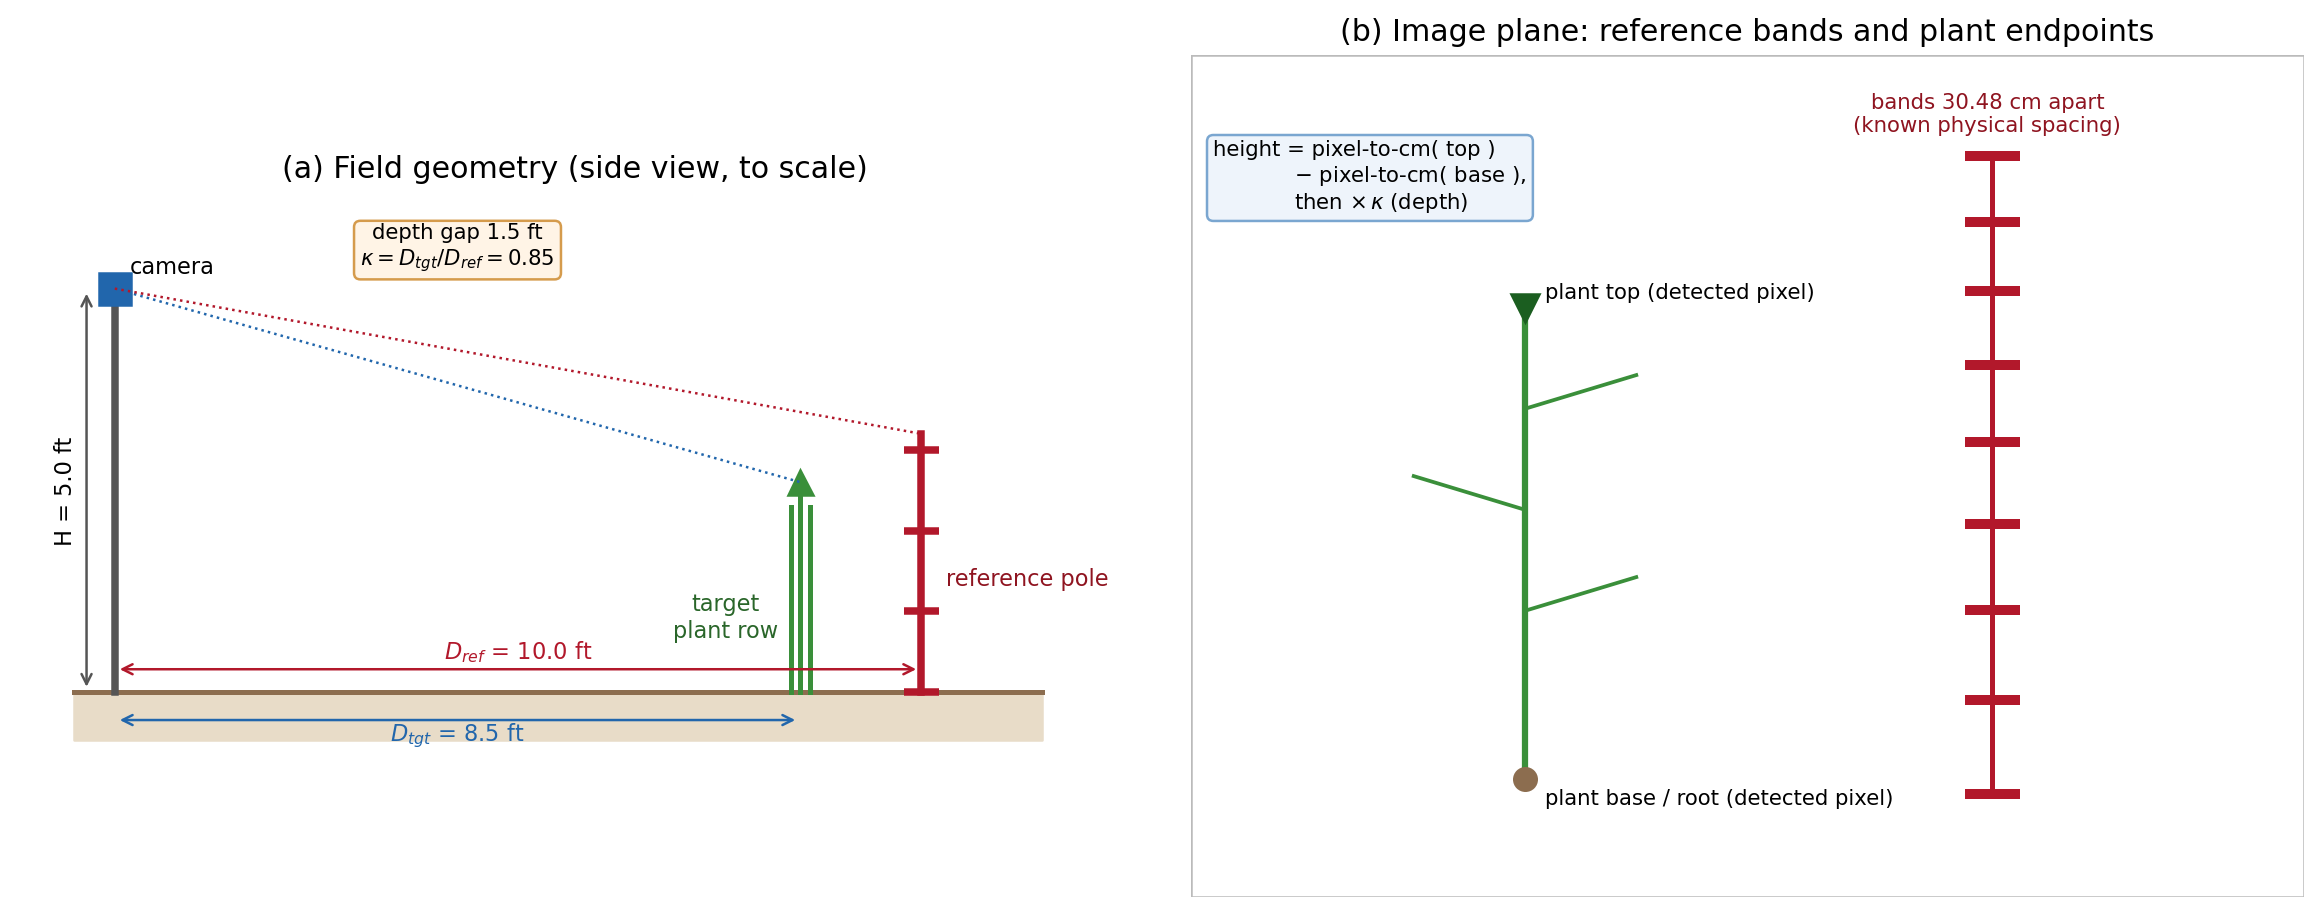
\includegraphics[width=\textwidth]{geometry_diagram.png}
\caption{Idealized calibration-transfer geometry. (a) Side view with the 2024--2025 camera at 5 ft, the target row at $D_{\mathrm{tgt}}=8.5$ ft, and the red-band reference at $D_{\mathrm{ref}}=10.0$ ft, giving $\kappa=0.85$. (b) Image-plane construction: the projective curve maps detected top and base rows onto the pole scale before the fixed depth factor is applied. The 30.48-cm labels refer to the red-band calibration pole, not the separate 2021 support poles.}
\label{fig:s-geometry}
\end{figure}

\section{Height-growth particle filter and exact predictive mixture}
\label{sec:s-mixture}

For elapsed time $\Delta_t$ in days, the implemented transition order is
\begin{align}
h_t^{(m)} &= \operatorname{clip}_{[0,450]}\!\left[
h_{t-1}^{(m)}+\Delta_t r_{t-1}^{(m)}
+\sigma_h\sqrt{\Delta_t}\,\epsilon_{h,t}^{(m)}\right],\\
r_t^{(m)} &= \operatorname{clip}_{[-4,15]}\!\left[
T\!\left(h_t^{(m)},r_{t-1}^{(m)}\right)
+\sigma_r\sqrt{\Delta_t}\,\epsilon_{r,t}^{(m)}\right],
\label{eq:s-transition}
\end{align}
where the innovations are independent standard normal variables. For the daily pole stream, $T(h,r)=r$. For the 2021 transferred-growth-field configuration, $T(h,r)=\widehat r(h)$, the nonparametric rate-versus-height field estimated from 2024--2025 image increments. Manual 2021 field heights do not enter $\widehat r$.

Conditional on height particle $h_t^{(m)}$, the observation law is
\begin{equation}
p(Y_t=y\mid h_t^{(m)})
=(1-\pi_t)\,\phi\!\left(y;h_t^{(m)},\sigma_t^2\right)
+\pi_t\,\phi\!\left(y;h_t^{(m)},\sigma_{\mathrm{out}}^2\right).
\label{eq:s-observation}
\end{equation}
Let $w_m^-$ be normalized particle weights after propagation and before observing $Y_t$. The exact one-step predictive density and cumulative distribution are
\begin{align}
p_t^-(y)
&=\sum_{m=1}^{M}w_m^-\left[
(1-\pi_t)\phi\!\left(y;h_t^{(m)},\sigma_t^2\right)
+\pi_t\phi\!\left(y;h_t^{(m)},\sigma_{\mathrm{out}}^2\right)
\right],\\
F_t^-(y)
&=\sum_{m=1}^{M}w_m^-\left[
(1-\pi_t)\Phi\!\left(\frac{y-h_t^{(m)}}{\sigma_t}\right)
+\pi_t\Phi\!\left(\frac{y-h_t^{(m)}}{\sigma_{\mathrm{out}}}\right)
\right].
\label{eq:s-predictive-cdf}
\end{align}
Predictive endpoints at probabilities 0.025, 0.05, 0.10, 0.25, 0.50, 0.75, 0.90, 0.95, and 0.975 solve $F_t^-(q_p)=p$ by numerical root finding. These quantiles provide central 50\%, 80\%, 90\%, and 95\% intervals. The predictive probability integral transform is $F_t^-(Y_t)$. The reported predictive standard deviation uses
\begin{equation}
\operatorname{Var}(Y_t\mid\mathcal I_{\leq t-1})
=\sum_m w_m^-\left(h_t^{(m)}-\bar h_t^-\right)^2
+(1-\pi_t)\sigma_t^2+\pi_t\sigma_{\mathrm{out}}^2.
\label{eq:s-predictive-variance}
\end{equation}
Equations~\ref{eq:s-predictive-cdf} and \ref{eq:s-predictive-variance} retain both mixture components. They replace the earlier normal approximation based only on latent-particle and inlier variances.

After $Y_t$ is observed, the weights are updated as
\begin{equation}
w_m \propto w_m^-\,p(Y_t\mid h_t^{(m)}),
\qquad \sum_m w_m=1.
\label{eq:s-weight-update}
\end{equation}
The posterior mean and interval for latent height are computed from these updated weights. A posterior interval therefore targets $h_t$ after the current image, whereas the predictive interval targets the next noisy image-derived measurement before it is observed. Coverage for those two targets is not interchangeable.

\begin{figure}[htbp]
\centering
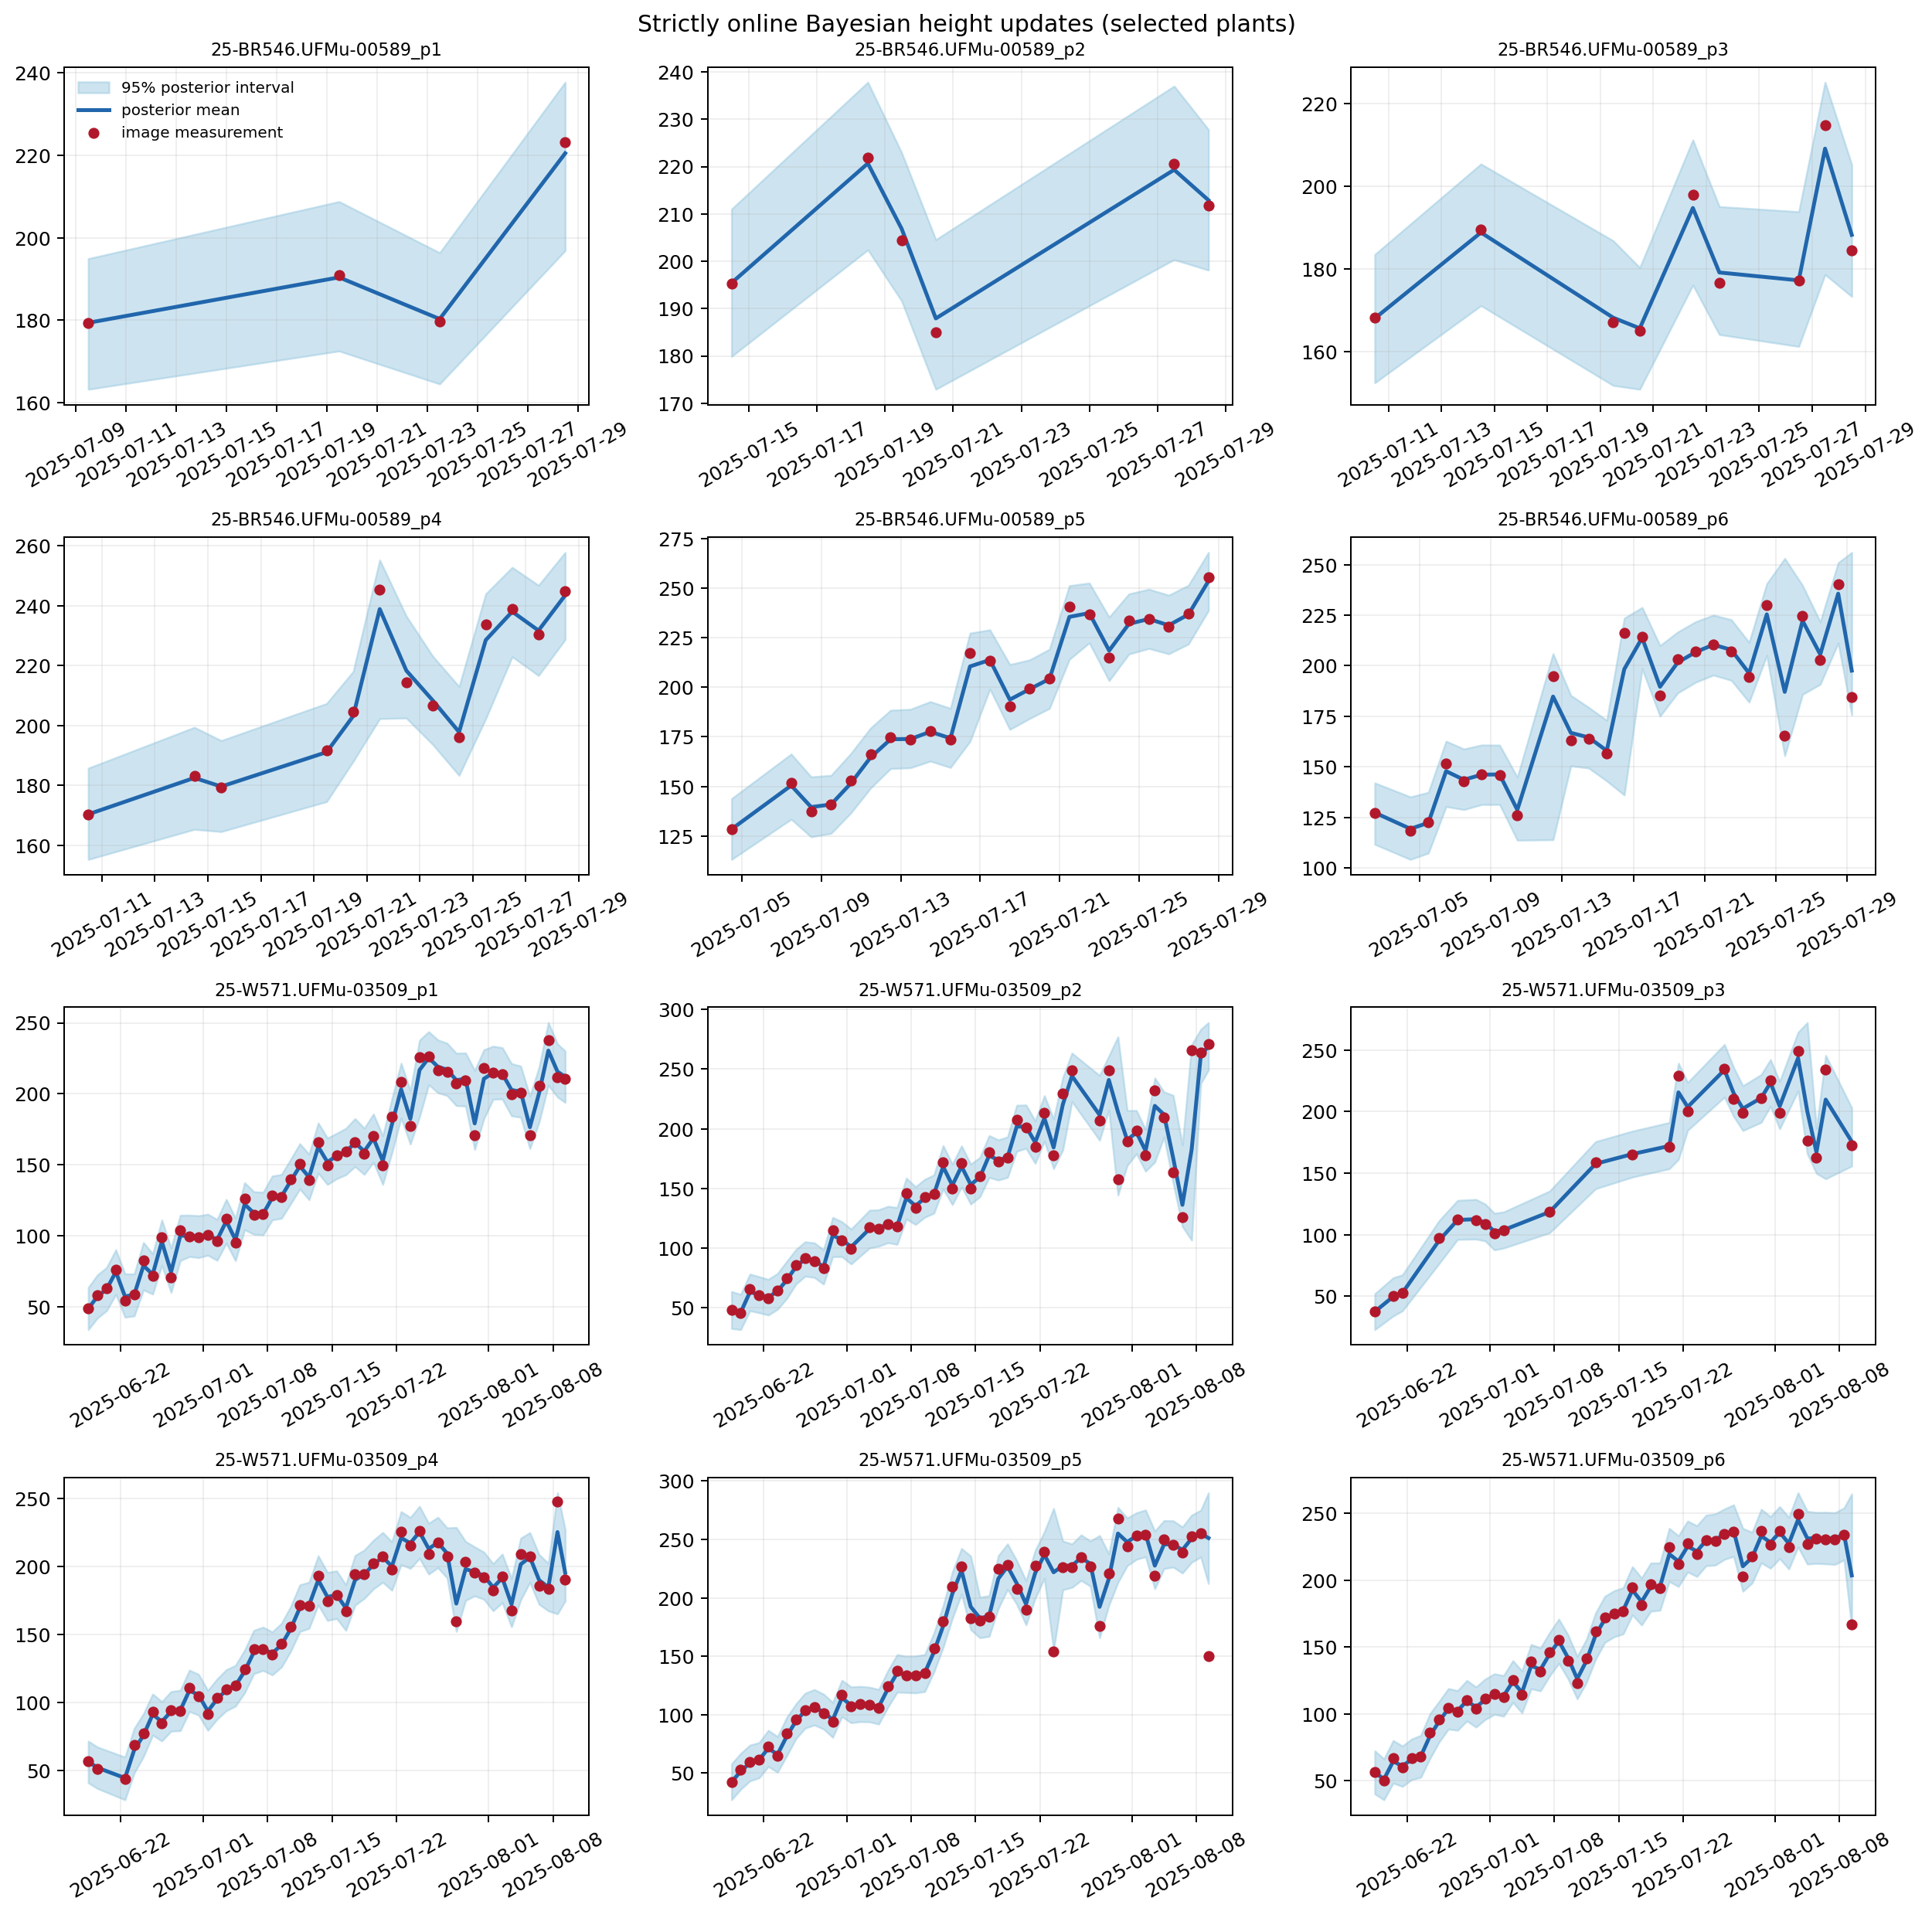
\includegraphics[width=0.88\textwidth]{bayesian_trajectories.png}
\caption{Selected 2025 daily pole-camera trajectories from the field-executed height-growth particle filter. Red points are depth-corrected image measurements, blue lines are posterior means after the corresponding image, and shading is the weighted 95\% latent-height posterior interval. Later observations initiate later updates; they do not retrospectively revise the plotted earlier estimates. The figure illustrates posterior behavior against image-derived measurements and is not validation against manual plant height.}
\label{fig:s-trajectories}
\end{figure}
\clearpage

\section{Secondary predictive-uncertainty transfer across years}
\label{sec:s-uncertainty}

This secondary analysis evaluates temporal transfer of predictive uncertainty for the next image-derived measurement. The 0.85 depth conversion changes every quantity expressed in centimeters. The corrected analysis therefore applies it to the image-derived height and its measurement standard deviation, and estimates the process and outlier scales from already corrected 2024 increments. The 2025 records are not used to estimate these values. Because plants were newly grown each season, the 2025 cohort is temporally later and subject-disjoint from 2024; no biological plant subject appears in both years. Over the complete quality-controlled stream, the unit-consistent predictive mean had mean absolute error \ForecastBayesMAE{} cm, mean log score \CalibratedLogScore{}, and weighted interval score \CalibratedWIS{} cm.

Table~\ref{tab:s-uncertainty} and Figure~\ref{fig:s-uncertainty} show calibration at multiple levels. On \UncertaintyTestN{} year-forward 2025 forecasts from \UncertaintyTestPlants{} evaluated plant tracks and \UncertaintyTestCameras{} cameras, the 95\% interval achieved \UncertaintyTestCoverageNinetyFive{}\% coverage with a \UncertaintyTestWidthNinetyFive{}-cm mean width. The 50\%, 80\%, and 90\% intervals covered \UncertaintyTestCoverageFifty{}\%, \UncertaintyTestCoverageEighty{}\%, and \UncertaintyTestCoverageNinety{}\%, respectively. This pattern is conservative at the lower levels even though the 95\% result is near nominal. Subject disjointness prevents repeated plants across years; it does not make repeated forecasts within a plant or camera independent. With only two test cameras, this analysis supports temporal transfer for those installations and does not establish broad camera generalization. The primary physical-height validation instead uses manual measurements across 12 stationary-camera rows.

\begin{table}[htbp]
\caption{Secondary temporal predictive-interval evaluation. Parameters for the unit-consistent model were estimated from 2024 only. Each target is the next image-derived measurement before it was observed.}
\label{tab:s-uncertainty}
\centering
\begin{tabular}{lrrrrr}
\toprule
Split & Forecasts & Cameras & Nominal (\%) & Coverage (\%) & Mean width (cm) \\
\midrule
2024 development & \UncertaintyDevN & \UncertaintyDevCameras & 50 & \UncertaintyDevCoverageFifty & \UncertaintyDevWidthFifty \\
 & & & 80 & \UncertaintyDevCoverageEighty & \UncertaintyDevWidthEighty \\
 & & & 90 & \UncertaintyDevCoverageNinety & \UncertaintyDevWidthNinety \\
 & & & 95 & \UncertaintyDevCoverageNinetyFive & \UncertaintyDevWidthNinetyFive \\
\addlinespace
2025 test & \UncertaintyTestN & \UncertaintyTestCameras & 50 & \UncertaintyTestCoverageFifty & \UncertaintyTestWidthFifty \\
 & & & 80 & \UncertaintyTestCoverageEighty & \UncertaintyTestWidthEighty \\
 & & & 90 & \UncertaintyTestCoverageNinety & \UncertaintyTestWidthNinety \\
 & & & 95 & \UncertaintyTestCoverageNinetyFive & \UncertaintyTestWidthNinetyFive \\
\bottomrule
\end{tabular}
\end{table}

\begin{figure}[htbp]
\centering
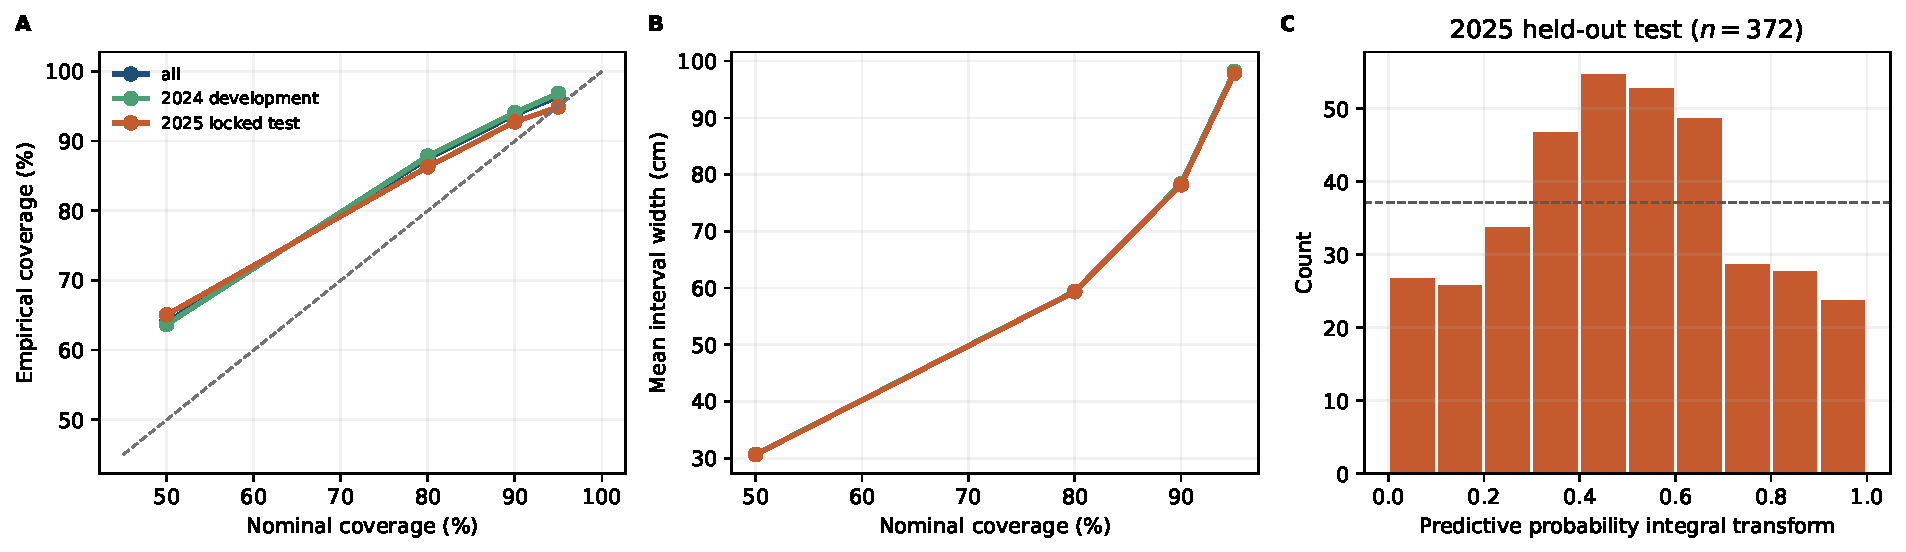
\includegraphics[width=0.9\textwidth]{uncertainty_calibration.pdf}
\caption{Secondary temporal evaluation of coverage and interval width for the unit-consistent predictive distribution. Parameters were estimated from the 2024 development cohort; the newly planted, subject-disjoint 2025 cohort was held out. The diagonal in the coverage panel marks exact nominal coverage. Points above the diagonal indicate conservative intervals.}
\label{fig:s-uncertainty}
\end{figure}

\section{Matched real-image candidate audit}
\label{sec:s-real-candidates}

The real-image audit uses cached candidates from the released 2021 pose checkpoint. Each temporal method receives identical candidates, confidence scores, association gates, fixed scale (0.415886 cm/pixel), and particle-filter settings. Human-mask root positions initialize the first image only. Subsequent associations use the running state; manual field height is reserved for scoring. The matched subset contains \RealAuditN{} plant-dates from \RealAuditTracks{} tracks in \RealAuditCameras{} cameras.

The post-detection and prior-in-candidate methods agreed on every selected candidate (Table~\ref{tab:s-real-candidates}). Their errors are consequently identical. This is a useful negative control: under these natural-image candidates and gates, there was no ambiguity for the height distribution to resolve. It cannot verify the accuracy gain seen in the controlled ambiguity simulation.

\begin{table}[htbp]
\caption{Real-image candidate audit. Manual field heights were used only for scoring.}
\label{tab:s-real-candidates}
\centering
\small
\setlength{\tabcolsep}{4pt}
\begin{tabular}{lrrr}
\toprule
Method & Signed error (cm) & MAE (cm) & RMSE (cm) \\
\midrule
Single frame & -9.55 & \RealAuditSingleMAE & \RealAuditSingleRMSE \\
Identical candidate plus post-detection filter & -9.27 & \RealAuditPostMAE & \RealAuditPostRMSE \\
Height prior in candidate scoring plus same filter & -9.27 & \RealAuditPriorMAE & \RealAuditPriorRMSE \\
\bottomrule
\end{tabular}
\end{table}

\clearpage

\section{All-plant mature-date results}
\label{sec:s-per-plant}

Table~\ref{tab:s-per-plant} lists the last available 2021 observation for every plant retained in the primary manual-reference validation. No plant is removed using image-minus-field residuals. The single-frame column is the archived geometrically scaled mask extent; the Bayesian column is the height-growth particle-filter posterior mean. The interval is the 2.5th to 97.5th percentile of the latent-height posterior after the endpoint image. Manual endpoint height is used for scoring and is not supplied to the filter.

\begin{longtable}{L{2.4cm}rrrr}
\caption{All \FieldPlants{} plants at their last available 2021 field date. Heights and interval endpoints are in centimeters.}\label{tab:s-per-plant}\\
\toprule
Plant & Manual field & Single frame & Bayesian mean & Bayesian 95\% interval \\
\midrule
\endfirsthead
\multicolumn{5}{l}{\textit{Table \thetable{} continued}}\\
\toprule
Plant & Manual field & Single frame & Bayesian mean & Bayesian 95\% interval \\
\midrule
\endhead
\midrule
\multicolumn{5}{r}{\textit{Continued on next page}}\\
\endfoot
\bottomrule
\endlastfoot
C\_004-p1 & 110.0 & 110.8 & 109.2 & [79.2, 142.4] \\
C\_004-p3 & 132.0 & 129.8 & 149.0 & [120.3, 178.9] \\
C\_004-p4 & 140.0 & 144.5 & 138.0 & [108.4, 169.2] \\
C\_005-p1 & 144.0 & 153.9 & 128.3 & [98.5, 158.7] \\
C\_005-p4 & 130.0 & 125.6 & 136.4 & [106.8, 167.3] \\
C\_005-p5 & 138.0 & 133.9 & 136.6 & [106.7, 167.7] \\
C\_009-p1 & 148.0 & 146.8 & 151.1 & [121.6, 182.2] \\
C\_009-p2 & 132.0 & 133.5 & 140.1 & [111.9, 170.8] \\
C\_009-p3 & 136.0 & 146.0 & 154.7 & [124.6, 185.4] \\
C\_010-p1 & 116.0 & 116.0 & 123.2 & [92.1, 157.1] \\
C\_010-p2 & 112.0 & 120.8 & 127.0 & [95.9, 161.0] \\
C\_010-p3 & 70.0 & 98.1 & 80.3 & [28.5, 136.8] \\
C\_011-p1 & 196.0 & 211.9 & 204.0 & [141.2, 239.5] \\
C\_011-p2 & 196.0 & 210.4 & 205.6 & [137.7, 244.5] \\
C\_011-p3 & 196.0 & 216.7 & 198.6 & [149.6, 231.2] \\
C\_021-p3 & 48.0 & 75.9 & 45.3 & [11.6, 79.1] \\
C\_021-p4 & 110.0 & 86.9 & 117.8 & [86.8, 159.0] \\
C\_024-p1 & 116.0 & 137.2 & 122.6 & [91.1, 157.4] \\
C\_024-p2 & 112.0 & 122.7 & 130.2 & [99.5, 164.1] \\
C\_024-p3 & 118.0 & 123.9 & 125.0 & [94.8, 158.8] \\
C\_029-p1 & 210.0 & 212.1 & 208.7 & [178.5, 238.0] \\
C\_029-p4 & 200.0 & 217.9 & 216.9 & [185.9, 246.8] \\
C\_029-p5 & 190.0 & 216.1 & 212.8 & [182.7, 242.6] \\
C\_032-p1 & 130.0 & 124.6 & 125.2 & [93.8, 158.6] \\
C\_032-p2 & 120.0 & 136.4 & 138.4 & [107.2, 170.6] \\
C\_032-p4 & 140.0 & 142.6 & 129.7 & [99.2, 164.6] \\
C\_037-p2 & 90.0 & 91.9 & 113.4 & [83.5, 145.5] \\
C\_037-p3 & 100.0 & 98.1 & 117.4 & [88.8, 148.8] \\
C\_037-p4 & 112.0 & 115.8 & 110.6 & [80.6, 144.4] \\
C\_038-p1 & 142.0 & 84.8 & 83.2 & [51.9, 116.8] \\
C\_039-p1 & 120.0 & 154.7 & 147.1 & [117.6, 176.6] \\
C\_039-p2 & 110.0 & 155.1 & 144.4 & [113.8, 176.6] \\
C\_039-p3 & 140.0 & 147.2 & 136.7 & [107.0, 167.5] \\

\end{longtable}

Across these \FieldEndpointN{} endpoints, single-frame mean absolute error was \FieldEndpointSingleMAE{} cm and the Bayesian mean absolute error was \FieldEndpointBayesMAE{} cm. The Bayesian signed error was +\FieldEndpointBayesBias{} cm. The stationary-camera-row bootstrap interval for the \FieldEndpointGain{}-cm paired mean-absolute-error reduction was \FieldEndpointGainLo{} to \FieldEndpointGainHi{} cm. These endpoint results are secondary because the interval is wide and includes zero; the main article uses all \FieldN{} plant-date records as its primary comparison.

\section{Data provenance and reproducibility}
\label{sec:s-reproducibility}

All paths below are relative to the \href{https://github.com/ChongWangStat/Bayesian-Longitudinal-Maize-Height}{public GitHub repository}.

\begingroup
\footnotesize
\setstretch{1.08}
\begin{longtable}{L{3.25cm}L{4.75cm}L{5.0cm}}
\caption{Data and result provenance for the revised submission.}\label{tab:s-provenance}\\
\toprule
Asset & Canonical path or source & Role and limitation \\
\midrule
\endfirsthead
\multicolumn{3}{l}{\textit{Table \thetable{} continued}}\\
\toprule
Asset & Canonical path or source & Role and limitation \\
\midrule
\endhead
\midrule
\multicolumn{3}{r}{\textit{Continued on next page}}\\
\endfoot
\bottomrule
\endlastfoot
2021 pole XML & \path{data/manual_annotations/poles_2021/C-*.xml} & Haoming Wang's human physical-reference annotations; one XML per camera row \\
2021 pole images & \path{data/raw/pole_calibration_images/} & All 61 curated images; confirmed duplicate omitted \\
Imported 2021 pole table & \path{data/processed/manual_poles_2021/manual_pole_annotations_2021.csv} & Trace endpoints, status, pixel length, and physical definition after duplicate removal \\
Pole definitions & \path{data/processed/manual_poles_2021/pole_definitions_2021.csv} & Documents 5-ft support length and distinguishes horizontal 35-in marks from red-band spacing \\
Daily image manifest & \path{data/processed/pole_camera_daily_manifest.csv} & As-of capture records, local/remote identifiers, and checksums \\
Released pose checkpoint & \path{models/maize_pose_2021_best.pt} & 2021 YOLO pose weights with SHA-256 checksum and model card \\
Curated-image pose candidates & \path{outputs/pose_candidates_annotation_set_2021/pose_candidates.csv} & Complete cache for all 61 released images \\
Automatic calibrations & \path{data/processed/automatic_pole_calibrations_daily.csv} & Candidate red-band fits and quality-control fields \\
Causal audit & \path{outputs/online_study/causality_audit_daily.json} & Prefix recomputation for cached detections through measurement assembly \\
Daily Bayesian output & \path{outputs/online_study/pole_camera_bayesian_daily_revised/online_bayesian_height_posteriors.csv} & Unit-consistent exact-mixture predictive and posterior summaries \\
Daily model settings & \path{outputs/online_study/pole_camera_bayesian_daily_revised/model_hyperparameters.json} & Complete saved particle-filter settings \\
2021 primary validation & \path{data/raw/heights_compare_2021.csv} & Archived image extents and 132 manual field measurements across 12 stationary-camera rows; raw-image-to-extent provenance remains incomplete \\
2021 canonical posterior & \path{outputs/filter_height_sam_2021/filtered_height_sam__phi1.0_plus_pole_growth_field.csv} & Input to all-plants and per-plant summaries \\
Primary field summary & \path{outputs/filter_height_sam_2021/all_plants_primary.json} & All-record and endpoint metrics with stationary-camera-row-cluster intervals \\
Detector-unit correction & \path{outputs/pixel_validation_2021/summary.json} & Recomputed centimeter metrics using 0.41588595 cm/pixel rather than the withdrawn field-regression conversion \\
Field baselines & \path{outputs/field_baselines_2021/} & Fixed causal comparators and row-cluster intervals \\
Real-image candidate audit & \path{outputs/real_image_candidate_ablation_2021/} & Matched candidate comparison with human truth used only for scoring \\
Generated manuscript values & \path{manuscript/numbers.tex} and \path{manuscript/per_plant_table.tex} & Programmatically generated values and per-plant table included by the submission source \\
\end{longtable}
\endgroup

\small
\enlargethispage{7\baselineskip}

The main regeneration sequence is shown below. The daily-chain shell script requires a Bash environment. The 2021 filter also requires the locally documented weather workbook used to create its five date-specific gust values.

\begin{verbatim}
python analysis/import_manual_poles_2021.py \
  --xml-dir data/manual_annotations/poles_2021 \
  --image-dir data/raw/pole_calibration_images \
  --output-dir data/processed/manual_poles_2021
bash analysis/run_daily_online_study.sh
python analysis/filter_on_height_sam_2021.py
python analysis/all_plants_primary_2021.py
python analysis/field_baseline_comparison_2021.py
python analysis/real_image_candidate_ablation_2021.py
python analysis/summarize_uncertainty_revision.py
python analysis/recalculate_pixel_validation_units.py
python manuscript/generate_numbers.py
# Regenerate the manuscript figures from the project root:
python analysis/plot_online_bayesian_workflow.py
python analysis/plot_pole_annotation_2021.py
python analysis/plot_calibration_validation.py
python analysis/plot_prior_in_detection_sim.py
python analysis/plot_field_validation_2021.py
python analysis/plot_geometry_diagram.py
\end{verbatim}

Particle-filter outputs store all settings and deterministic plant-specific seeds. The 20,000-replicate bootstrap seed is recorded in \path{all_plants_primary.json}. The release includes an MIT code license, a SHA-256 manifest, the final pose checkpoint, all 61 curated 2021 images, and the completed 199-trace human physical-reference audit. Non-code materials have no separate reuse license. The larger 2024--2025 raw-image archive and original cross-fitting image set are excluded, while the derived measurements needed to regenerate reported summaries are included.

\normalsize

\end{document}
